\newpage
\chapter{Midas}
\subsubsection{Eindimensionales Signal}
\label{chap:appendix_midas_ts}
\begin{figure}[h]
	\centering
	\subfloat[Ausrei�er-Typ Signal Drift\label{img:dailyDriftIso}]{
		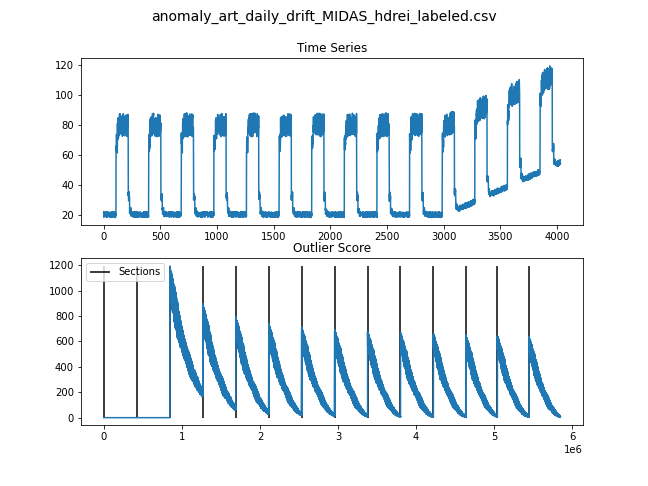
\includegraphics[width=0.5\textwidth]{fig/resultsMidasTS/anomaly_art_daily_drift_MIDAS_hdrei_labeled_result}}
	\subfloat[Ausrei�er-Typ Zunahme an Rauschen\label{img:increaseNoiseIso}]{
		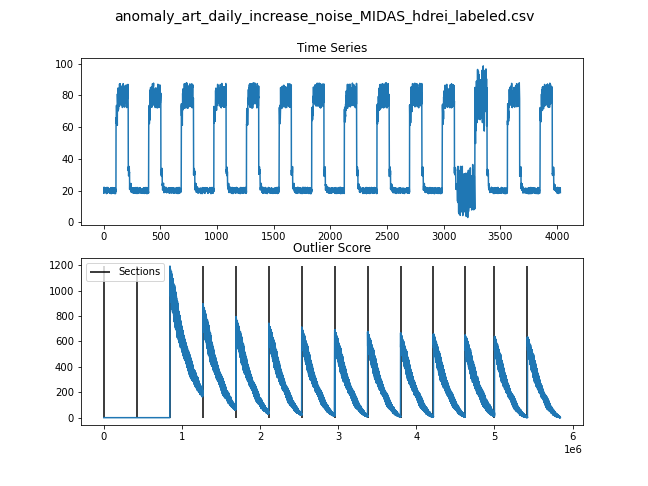
\includegraphics[width=0.5\textwidth]{fig/resultsMidasTS/anomaly_art_daily_increase_noise_MIDAS_hdrei_labeled_result}}
	\qquad
	\subfloat[Ausrei�er-Typ Einzelne Peaks\label{img:dailyPeaksIso}]{
		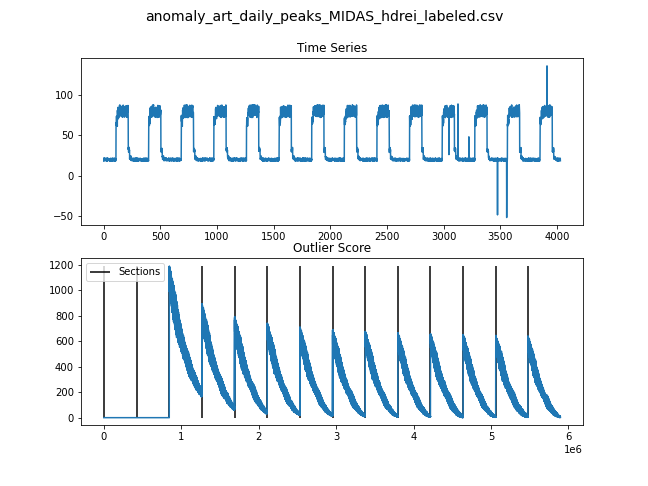
\includegraphics[width=0.5\textwidth]{fig/resultsMidasTS/anomaly_art_daily_peaks_MIDAS_hdrei_labeled_result}}
	\subfloat[Ausrei�er-Typ Frequenz�nderung\label{img:sequenceChangeIso}]{
		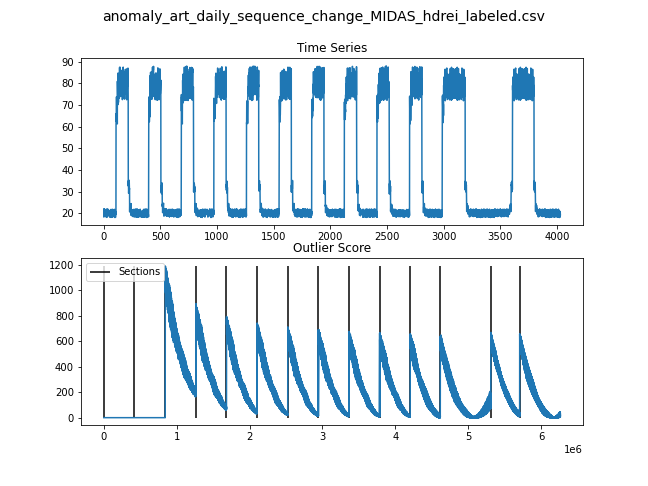
\includegraphics[width=0.5\textwidth]{fig/resultsMidasTS/anomaly_art_daily_sequence_change_MIDAS_hdrei_labeled_result}}
	\qquad
	\label{img:midaspictures1}
\end{figure}
\begin{figure}\ContinuedFloat
	\subfloat[Ausrei�er-Typ Kontinuierliche Zunahme der Amplitude\label{img:ampRiseIso}]{
		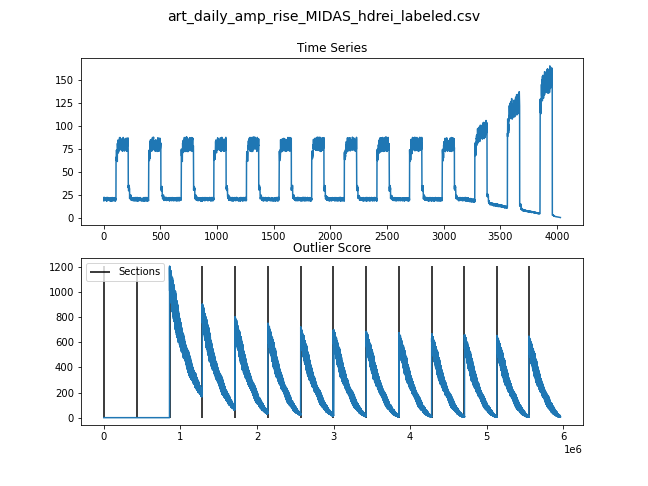
\includegraphics[width=0.5\textwidth]{fig/resultsMidasTS/art_daily_amp_rise_MIDAS_hdrei_labeled_result}}
	\subfloat[Ausrei�er-Typ Zyklus-Aussetzer\label{img:flatmiddleIso}]{
		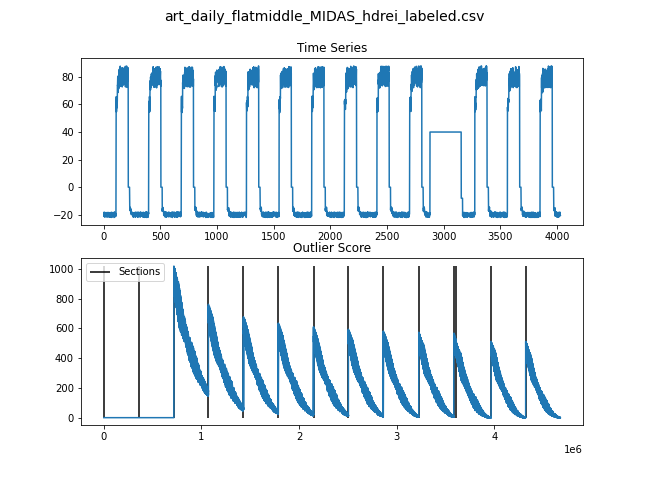
\includegraphics[width=0.5\textwidth]{fig/resultsMidasTS/art_daily_flatmiddle_MIDAS_hdrei_labeled_result}}
	\qquad
	\subfloat[Ausrei�er-Typ Zyklus mit geringerer Amplitude\label{img:jumpsdownIso}]{
		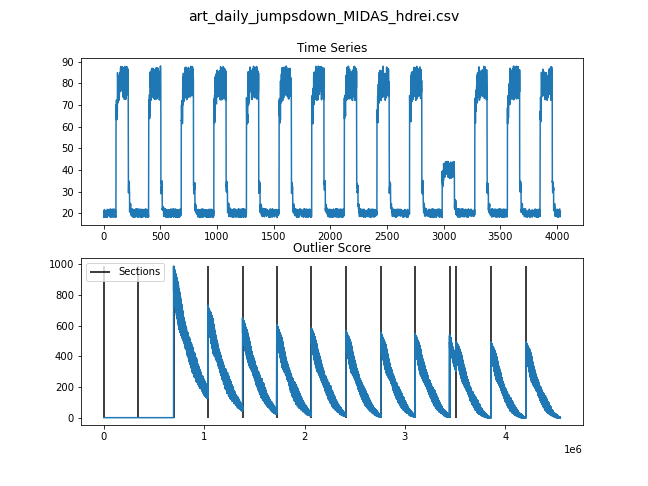
\includegraphics[width=0.5\textwidth]{fig/resultsMidasTS/art_daily_jumpsdown_MIDAS_hdrei_result}}
	\subfloat[Ausrei�er-Typ Zyklus mit h�herer Amplitude\label{img:jumpsupIso}]{
		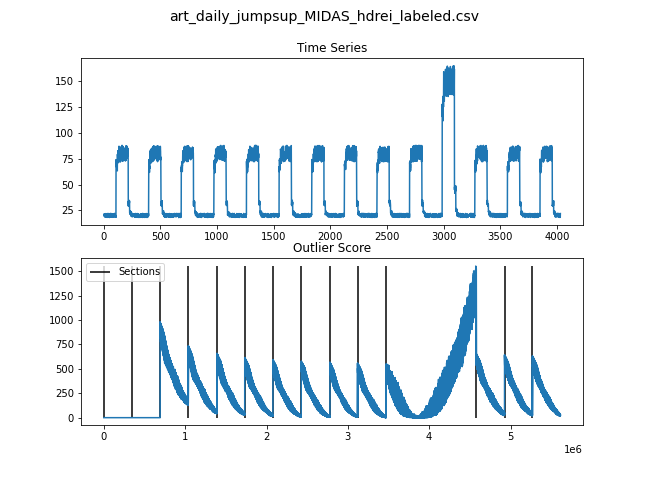
\includegraphics[width=0.5\textwidth]{fig/resultsMidasTS/art_daily_jumpsup_MIDAS_hdrei_labeled_result}}
	\qquad
	\subfloat[Ausrei�er-Typ Signal-Aussetzer\label{img:nojumpIso}]{
		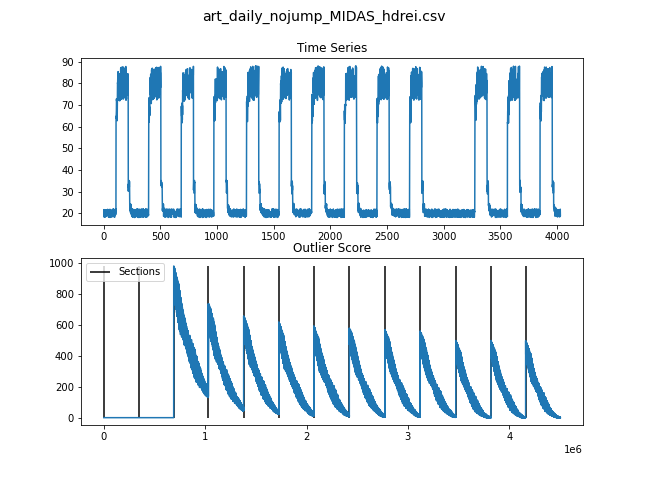
\includegraphics[width=0.5\textwidth]{fig/resultsMidasTS/art_daily_nojump_MIDAS_hdrei_result}}
	\label{img:midaspictures2}
\end{figure}